\documentclass[12pt,a4paper]{article}
\usepackage{vmargin}
\setmarginsrb{1.0in}{1.0in}{1.0in}{1.0in}{0mm}{0mm}{0mm}{10mm}

\usepackage{amsfonts,amsmath,amssymb}
\usepackage{amsthm}
\usepackage{graphicx}
\usepackage{amsmath}
\usepackage{xcolor}
%\usepackage{ngerman}
\usepackage{listings}
\usepackage[utf8]{inputenc}
%\usepackage[T1]{fontenc}
\usepackage{comment}
\usepackage{algorithm}
\usepackage{hyperref}
%%\usepackage{algpseudocode}
\renewcommand*\thealgorithm{}
\usepackage{algorithmic}
\usepackage{amsmath}

\newcommand{\N}{\mathbb{N}}
\newcommand{\R}{\mathbb{R}}
\renewcommand{\O}{\mathcal{O}}
\usepackage{mathtools}

\newtheorem{theorem}{Theorem}
\newtheorem{lemma}{Lemma}
\newtheorem{corollary}[theorem]{Corollary}
\newtheorem{conjecture}{Conjecture}
\newtheorem{fact}[theorem]{Fact}
%\newtheorem{proposition}[theorem]{Proposition}
\newtheorem{observation}{Observation}
%\newtheorem{notation}[theorem]{Notation}
\newtheorem{remark}{Remark}
\newtheorem{claim}{Claim}
\newtheorem{definition}{Definition}
%\theoremstyle{definition}
%\newtheorem{problem}[theorem]{Problem}
\newtheorem{example}{Example}
%\renewcommand{\qedsymbol}{\rule{1mm}{1mm}}
\newcommand\independent{\protect\mathpalette{\protect\independenT}{\perp}}
\def\thesection{\alph{section}}

\setlength{\parindent}{0pt}


\begin{document}

\noindent
\begin{minipage}{0.66\textwidth}
Hasso Plattner Institute Potsdam\\
\\
Seminar on Nature Inspired Algorithms\\ Summer 2017\\
Potsdam, \today
\end{minipage}
~
\begin{minipage}{0.30\textwidth}

\includegraphics[width=\textwidth]{../homework_template/Hasso_Plattner_Institut_Logo}
\end{minipage}


\begin{center}
 {\LARGE \textbf{Homework 1}}
 \vspace*{0.5cm}
\end{center}
%%%%%%%%%%%%%%%%%%%%%%%%%%%%%%%%%%%%%%%%%%%


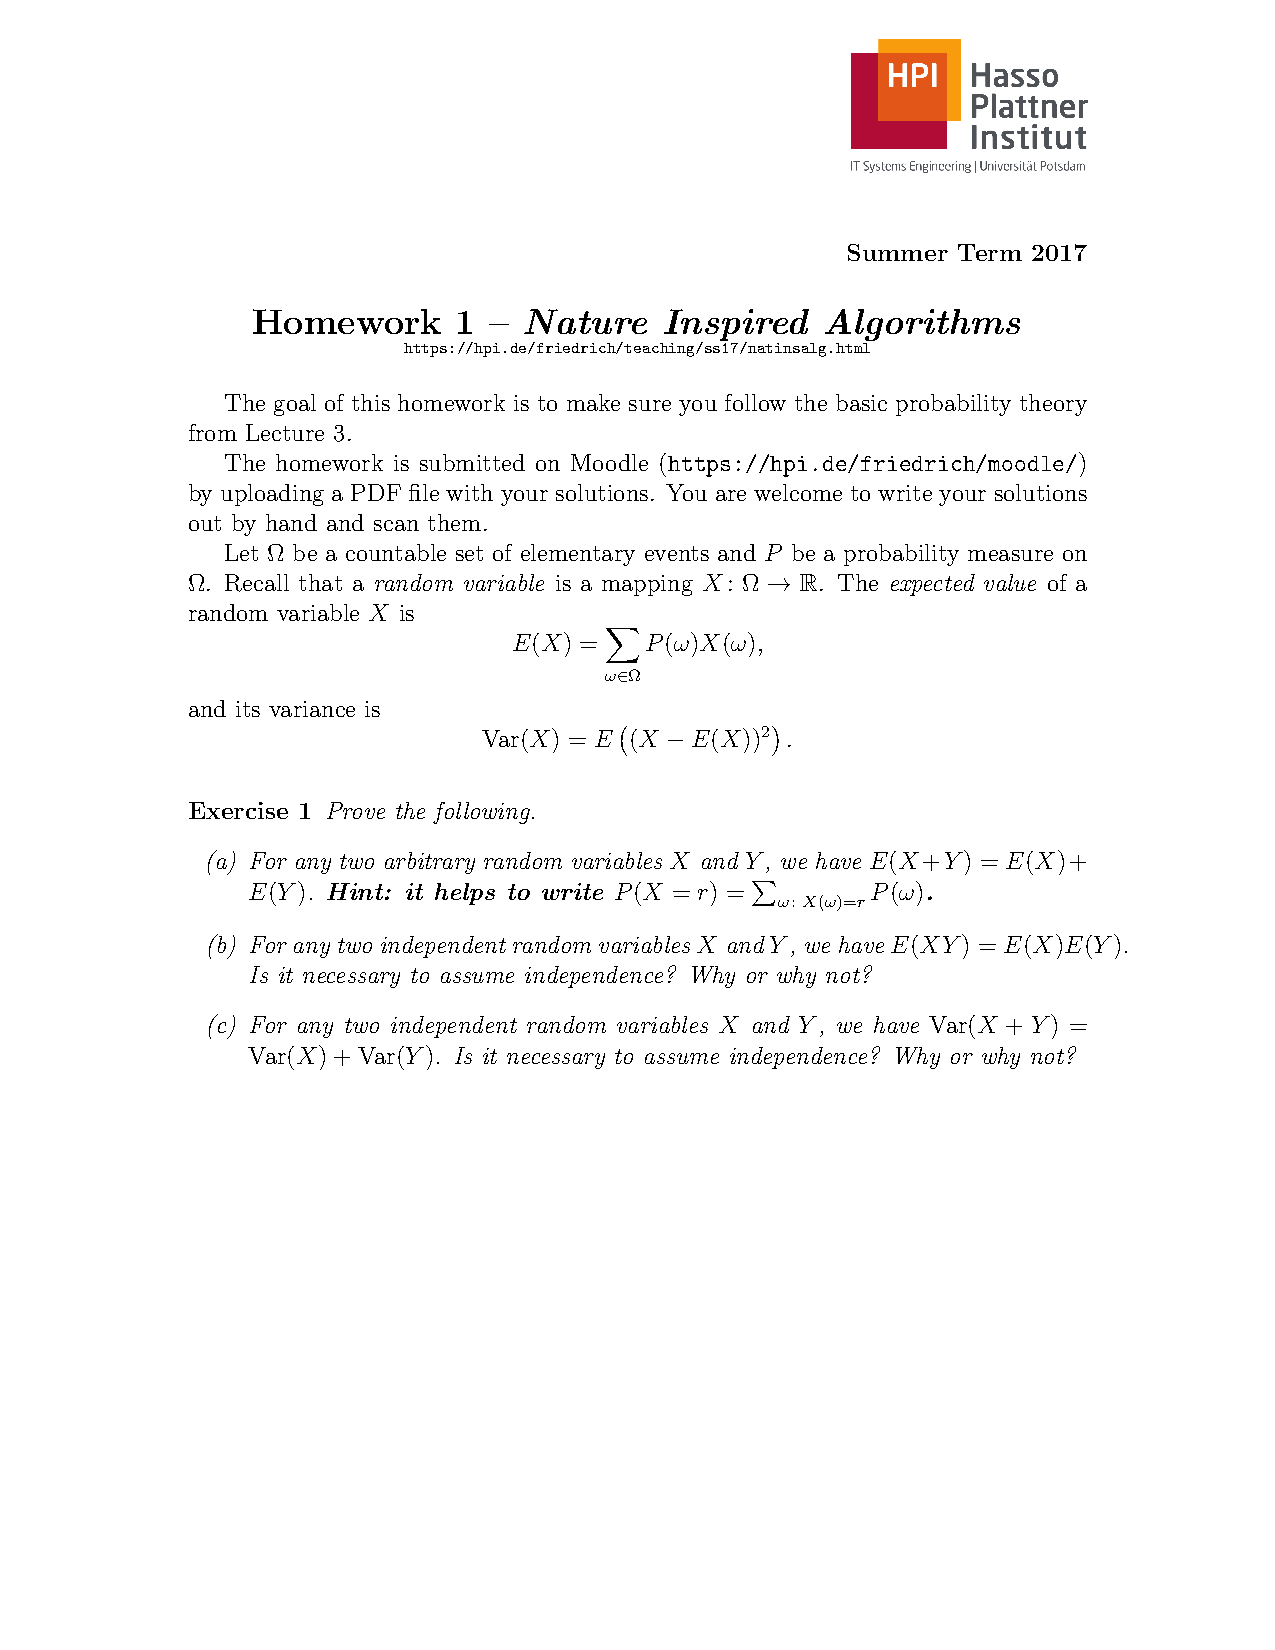
\includegraphics[clip, trim=0.5cm 2.5cm 0.5cm 4cm, width=0.99\textwidth]{homework01.pdf}

\section{}
\begin{align}
E(X+Y) &= \sum_{x \in \mathbb{R}}{}\sum_{y \in \mathbb{R}}{(x+y)P(X=x, Y=y)} \\
&= \sum_{x \in \mathbb{R}}{}\sum_{y \in \mathbb{R}}{x \cdotP P(X=x, Y=y)} + \sum_{x \in \mathbb{R}}{}\sum_{y \in \mathbb{R}}{y \cdotP P(X=x, Y=y)} \\
&= \sum_{x \in \mathbb{R}}{x}\sum_{y \in \mathbb{R}}{P(X=x, Y=y)} + \sum_{y \in \mathbb{R}}{y}\sum_{x \in \mathbb{R}}{P(X=x, Y=y)} \\
&= \sum_{x \in \mathbb{R}}{x}{P(X=x)} + \sum_{y \in \mathbb{R}}{y}{P(Y=y)} \\
&= E(X) + E(Y) \blacksquare
\end{align}

\section{}
\begin{align}
E(XY) &= \sum_{x \in \mathbb{R}}{}\sum_{y \in \mathbb{R}}{xy \cdot P(X=x, Y=y)} \\
&= \sum_{x \in \mathbb{R}}{x}\sum_{y \in \mathbb{R}}{y \cdot P(X=x, Y=y)} \\
% P(X=x, Y=y) = P(X=x)P(Y=y) \text{ if } X \independent Y\\
&= \sum_{x \in \mathbb{R}}{x}\sum_{y \in \mathbb{R}}{y \cdot P(X=x)P(Y=y)} \\
&= \sum_{x \in \mathbb{R}}{x}{P(X=x)}\sum_{y \in \mathbb{R}}{y}{P(Y=y)} \\
&= E(X)E(Y)
\end{align}
For arbitrary random variables X and Y the equation $E(XY) = E(X)E(Y)$ only always holds if X $\independent$ Y since $P(X=x, Y=y)$ is always $P(X=x)P(Y=y)$ in that case which is required during the proof. Thus, we have to assume independence. \blacksquare

\section{}
\begin{align}
% \mathcal \left \text{ if } $$X \independent Y$$ \text{ : } \right & \mathcal \left $$E((X+Y)^2) % - (E(X+Y))^2$$ \right \\
{Var(X+Y)} &= $$E((X+Y)^2) - E(X+Y)^2$$ \\
& = \sum_{x \in \mathbb{R}}{}\sum_{y \in \mathbb{R}}{(x+y)^2 \cdot P(X=x, Y=y)} - (E(X+Y))^2 \\
& = \sum_{x \in \mathbb{R}}{}\sum_{y \in \mathbb{R}}{x^2 \cdot P(X=x, Y=y)}
  + \sum_{x \in \mathbb{R}}{}\sum_{y \in \mathbb{R}}{2xy \cdot P(X=x, Y=y)} \\
& + \sum_{x \in \mathbb{R}}{}\sum_{y \in \mathbb{R}}{y^2 \cdot P(X=x, Y=y)}
  - (E(X))^2 - 2E(X)E(Y) - (E(Y))^2 \\
& = \sum_{x \in \mathbb{R}}{}{x^2 \cdot P(X=x)} - (E(X))^2
  + \sum_{y \in \mathbb{R}}{}{y^2 \cdot P(Y=y)} - (E(Y))^2 \\
& + \sum_{x \in \mathbb{R}}{}\sum_{y \in \mathbb{R}}{2xy \cdot P(X=x, Y=y)} - 2E(X)E(Y) \\
& = E(X^2) - (E(X))^2 + E(Y^2) - (E(Y))^2 + 2(E(XY) - E(X)E(Y)) \\
& = Var(X) + Var(Y) + 2Cov(X, Y)
\end{align}
For arbitrary random variables X and Y the equation $Var(X+Y) = Var(X) + Var(Y)$ only always holds if X $\independent$ Y since $Cov(X, Y)$ is always 0 in that case. Thus, we have to assume independence. \blacksquare

\end{document}
